documentclass[tikz]{standalone}
\usetikzlibrary{calc}
\tikzset{
  myarrow/.style={->},
  sys/.pic={
    \draw[myarrow,#1] (-0.65,-0.65) -- (-0.65,0.65);
    \draw[myarrow,#1] (0.65,-0.65) -- (0.65,0.65);
    \draw[myarrow,#1] (-0.65,-0.65) -- (0.65,-0.65);
    \node at (-0.65,0.35) {$p^{(1)}$};
    \node at (0.35,-0.65) {$r^{(1)}$};
    \node at (0.65,0.35) {$p^{(2)}$};
    \node at (-0.35,0.65) {$r^{(2)}$};
  },
  sysneg/.pic={
    \draw[myarrow,-#1] (-0.65,-0.65) -- (-0.65,0.65);
    \draw[myarrow,-#1] (0.65,-0.65) -- (0.65,0.65);
    \draw[myarrow,-#1] (-0.65,-0.65) -- (0.65,-0.65);
    \node at (-0.65,0.35) {$p^{(1)}$};
    \node at (0.35,-0.65) {$r^{(1)}$};
    \node at (0.65,0.35) {$p^{(2)}$};
    \node at (-0.35,0.65) {$r^{(2)}$};
  },
  syscol/.style={
    sys/.append style={fill=#1},
    sysneg/.append style={fill=#1}
  },
  syscol/.default=none,
}
\begin{document}
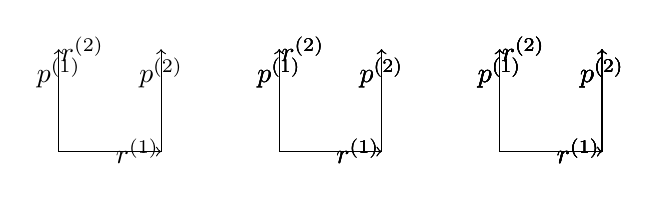
\begin{tikzpicture}[scale=0.7]
  \path (0,0) pic {sys} coordinate (A1);
  \path (4,0) pic {sys} coordinate (A2);
  \path (8,0) pic {sys} coordinate (A3);
  \path[xshift=4cm] (A2) pic {sys} coordinate (B1);
  \path[xshift=4cm] (A3) pic {sysneg} coordinate (B2);
  \path[xshift=4cm] (B2) pic {sysneg} coordinate (B3);
  \path[xshift=-4cm] (A2) pic {sysneg} coordinate (C1);
  \path[xshift=-4cm] (A3) pic {sys} coordinate (C2);
  \path[xshift=-4cm] (C2) pic {sys} coordinate (C3);
  \path[dotted] (B1|-A1) -- (B1|-A3);
  \path[dotted] (B2|-A1) -- (B2|-A3);
  \path[dotted] (C1|-A1) -- (C1|-A3);
\end{tikzpicture}
\end{document}